\section{*Two-flavour \chpt\ to leading order}
\label{section: two-flavor chpt to leading order}


\subsection{Paramterization}
\label{subsection: parametrization}

In this section, we will assume $N_f = 2$, which means the generators are $T_a = \frac{1}{2} \tau_a$, where $\tau_a$ are the Pauli Matrices, as described in \autoref{section: algebra bases}.
The quark mass matrix is
%
\begin{equation}
    \label{two-flavor mass matrix}
    m = 
    \begin{pmatrix}
        m_u & 0 \\ 
        0 & m_d 
    \end{pmatrix}.
\end{equation}
%
We define $\bar m^2 = B_0 (m_u + m_d)$ and $\Delta m^2 = B_0(m_u - m_d)$, so that when we set the scalar current $s$ equal to the quark masses, and the pseudoscalar current to zero, we get
%
\begin{equation}
    \label{chi definition}
    \chi = \bar m^2 \one + \Delta m^2 \tau_3,
\end{equation}


For $j = 0$, the ground state is by assumption $\Sigma = \one$, the vacuum, and we can use the paramterization
\begin{equation}
    \label{vacuum parametrization}
    \Sigma(x) = \exp{i \frac{\pi_a\tau_a}{f}},
\end{equation}
%
where $f$ is the bare pion decay constant, $\pi_a$ are the three Goldstone bosons, a set of real functions of space-time.
This ensures that $\pi = 0$ corresponds to the vacuum.
If we perform an infinitesimal isospin transformation, and assume $\pi/f$ small, then
%
\begin{equation}
    \Sigma \rightarrow U_V \Sigma U_V^\dagger
    =
    \left(1 + i \eta_a \frac{1}{2} \tau_a\right)
    \left(1 + i \frac{1}{f} \pi_b  \tau_b\right)
    \left(1 - i \eta_c \frac{1}{2} \tau_c\right)
    =
    1 + i\frac{1}{f}\pi_a (\delta_{ac} + i \eta_b \epsilon_{abc}) \tau_c,
\end{equation}
%
or
\begin{equation}
    \pi_a \rightarrow (\delta_{ac} + i \eta_b \epsilon_{abc}) \pi_c.
\end{equation}
%
The generators of $\pi_a$ under isospin-transformations are thus the adjoint representation of $\mathfrak{su}(2)$, and they form an isospin triplet.
For $\eta_1 = \eta_2 = 0$, i.e. transformations generated by $\tau_3$, $\pi_3$ is invariant, which means that it has quantum number $I_3 = 0$.\footnote{Authors differe if they define $\sqrt 2 \pi^\pm = \pi_1 \pm i \pi_2$, or with opposite signs. We choose the former, so that $\pi_+ \ket{0}$ is the state with the quantum numbers of the positive pion.}
$\pi_1$ and $\pi_2$ do not have a definite value of the third component of isospin, but rather for the first and second component.
They are related to the observed, charged pions $\pi^+$ and $\pi^-$ by~\cite{schererIntroductionChiralPerturbation2002}
\begin{equation}
    \pi_a\tau_a
    = 
    \begin{pmatrix}
        \pi_3 & \pi_1 - i \pi_2 \\
        \pi_1 + i \pi_2 & - \pi_3
    \end{pmatrix}
    = 
    \begin{pmatrix}
        \pi^0 & \sqrt{2} \pi^- \\
        \sqrt 2 \pi^+ & - \pi^0
    \end{pmatrix},
\end{equation}
%
where $\pi^\pm$ has a third isospin-component of $I_3 = \pm1$.
For non-zero isospin chemical potential, however, we expect that the ground state may be rotated away from the vacuum.
To find what the new ground state is, we have to minimize the Hamiltonian.



\subsection{Leading order Lagrangian}
\label{section: leading order}

The leading order Lagrangian in Winberg's power counting scheme, with $e = 0$, is
%
\begin{equation}
    \label{leading order two-flavor chpt lagrangian}
    \Ell_2 = 
    \frac{1}{4} f^2 \Tr{\nabla_\mu \Sigma (\nabla^\mu \Sigma)^\dagger}
    + \frac{1}{4} f^2 \Tr{\chi^\dagger \Sigma + \Sigma^\dagger \chi}.
\end{equation}
%
The external source currents are
\begin{align}
    \nabla_\mu \Sigma &= \partial_\mu \Sigma - i [v_\mu, \Sigma],
    \quad v_\mu = \frac{1}{2} \mu_I \delta_\mu^0 \tau_3.
\end{align}
To incorporate a finite isospin density, we must parametrize the Goldstone manifold differently than in the vacuum.
We follow the analysis in~\autocite{adhikariTwoflavorChiralPerturbation2019}.
We assume the ground state is independent of space, $\pi_a(x) = \pi_a^0$, and write it as
\begin{equation}
    \Sigma_\alpha 
    :=
    \exp{i \alpha n_a \tau_a}
    = 
    \cos \alpha + i n_a \tau_a \sin \alpha,
\end{equation}
%
where
\begin{equation}
    \alpha = \frac{1}{f} \sqrt{\pi^0_a \pi^0_a}, \quad
    n_a = \frac{\pi^0_a}{\sqrt{\pi^0_a \pi^0_a}}.
\end{equation}
%
With this, the covariant derivative is $\nabla_\mu \Sigma_\alpha = - iv^a_\mu [\tau_a, \Sigma_\alpha]$, and the two terms in the first order Lagrangian are
\begin{align}
    \Tr{\nabla_\mu \Sigma_\alpha  (\nabla^\mu \Sigma_\alpha)^\dagger}
    & = 2 \mu_I^2 (n_1^2 + n_2^2) \sin^2 \alpha, \quad
    \Tr{\chi^\dagger \Sigma_\alpha + \Sigma_\alpha^\dagger \chi}
    = 4 \bar m^2 \cos \alpha.
\end{align}
%
We see that, to first order, all results are independent of $\Delta m$.
To find the new ground state, we minimize the Hamiltonian density.
With the assumption that the fields are constant, the first order Hamiltonian density is
\begin{equation}
    \He_2 = - \Ell_2 = 
    - f^2 
    \left[
        \bar m^2 \cos\alpha 
        + \frac{1}{2} \mu_I^2 (n_1^2 + n_2^2 ) \sin^2 \alpha
    \right]
\end{equation}
%
For $\mu_I = 0$, this is independent of $n_a$, and minimized by $\alpha = 0$.
Now, as $n_i n_i = 1$, we have that $n_1^2 + n_2^2 = 1 - n_3^2$.
This means that, for $\mu_I \neq 0$, the energy is minimized by $n_3 = 0$.
We can write $n_1 = \cos \phi$, $n_2 = \sin \phi$, for some real number $\phi$, which gives the ground state
\begin{equation}
    \Sigma_\alpha 
    = \one \cos \alpha  + i ( \tau_1 \cos \phi + \tau_2 \sin \phi) \sin \alpha .
\end{equation}
%
We can choose, without loss of generality, $\phi = 0$~\autocite{sonQCDFiniteIsospin2000}.
This corresponds to a change of basis of $\lie{su}{2}$, $\tau_1 \rightarrow \tilde \tau_1 = \tau_1 \cos \phi + \tau_2 \sin \phi$ and $\tau_2 \rightarrow \tilde \tau_2 = - \tau_1 \sin \phi + \tau_2 \cos \phi$.
With this, the new ground state is
%
\begin{equation}
    \label{general groundstate}
    \Sigma_\alpha = \exp{i \alpha \tau_1}
\end{equation}
%
Any exited state is a transformation of the ground state by $\Lie{SU}{2}_A$.
For $\mu_I = 0$, this corresponds to 
\begin{equation}
    \Sigma(x) = U_R(x) \Sigma_0 U_L^\dagger(x) = U(x) \Sigma_0 U(x).
\end{equation}
%
where
\begin{equation}
    U(x) = \exp{i \frac{\tau_a\pi_a(x)}{2f}}.
\end{equation}
%
We see that this recovers the parametrization \autoref{vacuum parametrization}.
For $\mu_I \neq 0$, the ground state may be shifted, and so $U(x)$ must be too.
The groundstate transforms as
\begin{equation}
    \Sigma_0 \rightarrow \Sigma_\alpha 
    = \hat U_L \Sigma_0 \hat U_R^\dagger = A_\alpha \Sigma_0 A_\alpha.
\end{equation}
%
where
\begin{equation}
    A_\alpha : = \exp{i \frac{1}{2} \alpha \tau_1} 
    = \cos \frac{\alpha}{2} + i \tau_1 \sin\frac{\alpha}{2}.
\end{equation}
%
This induces the following transformations for the fluctuations,
\begin{align}
    U_L & \rightarrow \hat U_L U_L \hat U_L^\dagger = A_\alpha U_L A_\alpha^\dagger, \\
    U_R & \rightarrow \hat U_R U_R \hat U_R^\dagger = A_\alpha^\dagger U_R A_\alpha.
\end{align}
%
The new parametrization is thus
\begin{align}
    \label{sigma}
        \Sigma(x) = A_\alpha [U(x) \Sigma_0 U(x)] A_\alpha.
\end{align}
%
With this, we can expand the first order Lagrangian, \autoref{leading order two-flavor chpt lagrangian}, in powers of $\pi/f$
We will use this expansion to calculate the free energy density.
Expanding $\Sigma$ to $\Oh \left((\pi/f)^5\right)$, we get
\begin{align}
    \Sigma =
     \left(
        1 
        - \frac{\pi_a^2}{2f^2}
        + \frac{\pi_a^2\pi_b^2}{24f^4}
    \right)
    (\cos{\alpha} + i \tau_1 \sin{\alpha})
    +
    \left(
        \frac{\pi_a}{f} 
        - \frac{\pi_b^2\pi_a}{6f^3} 
    \right)
    \left(
        i\tau_a - 2i \delta_{a1}\tau_1\sin^2{\frac{\alpha}{2}} - \delta_{a1} \sin{\alpha}
    \right).
    \label{expansion of sigma}
\end{align}
%

The kinetic term in the \chpt\, Lagrangian is
\begin{equation}
    \nabla_\mu \Sigma (\nabla^\mu \Sigma)^\dagger 
    = \partial_\mu \Sigma \partial^\mu \Sigma^\dagger 
    - i \left(\partial_\mu \Sigma [v^\mu, \Sigma^\dagger] - \hc \right)
    - [v_\mu,\Sigma][v_\mu, \Sigma^\dagger].
    \label{kinetic term}
\end{equation}
%
Using \autoref{expansion of sigma} we find the expansion of the constitutive parts of the kinetic term to be
\begin{align}
    \notag
    \partial_\mu \Sigma 
    = &
    \left[
        \left(
            \frac{-1}{f^2}
            + \frac{\pi_b^2}{6f^4}
        \right)
        (\pi_a \partial_\mu \pi_a)
        \cos{\alpha}
        - 
        \left(
            \frac{\partial_\mu \pi_1}{f} 
            - \frac{\pi_b^2 \partial_\mu\pi_1
            + 2 \pi_1 \pi_b \partial_\mu\pi_b}{6f^3} 
        \right)
        \sin{\alpha}
    \right]
    \\ \notag 
    - &
    \left[
        \left(
            \frac{-1}{f^2}
            + \frac{\pi_b^2}{6f^4}
        \right)
        (\pi_a \partial_\mu \pi_a)
        \sin{\alpha}
        - \left(
        \frac{\partial_\mu \pi_1}{f} 
        - \frac{\pi_b^2 \partial_\mu\pi_1
        + 2 \pi_1 \pi_b \partial_\mu\pi_b}{6f^3}
        \right)
        2 \sin^2{\frac{\alpha}{2}}
    \right]
    i \tau_1 \\ \label{Sigma derivative}
    +& 
    \left(
        \frac{\partial_\mu \pi_a}{f} 
        - \frac{\pi_b^2 \partial_\mu\pi_a 
        + 2 \pi_a \pi_b \partial_\mu\pi_b}{6f^3} 
    \right)
    i \tau_a,
\end{align}
%
and
\begin{align}
    % \notag
    [v_\mu,\Sigma]
    & =
    -\mu_I \delta^0_\mu
    \left\{
        \left[
        \left(
            1 
            - \frac{\pi_a^2}{2f^2}
            + \frac{\pi_a^2\pi_b^2}{24f^4}
        \right)
        \sin{\alpha}
        + 
        \left(
            \frac{\pi_1}{f} 
            - \frac{\pi_b^2\pi_1}{6f^3} 
        \right) \cos{\alpha}
        \right]
         \tau_2
        -
        \left(
            \frac{\pi_2}{f} 
            - \frac{\pi_b^2\pi_2}{6f^3} 
        \right)
        \tau_1
    \right\}.
    \label{sigma commutator}
\end{align}
%
Combining \autoref{Sigma derivative} and \autoref{sigma commutator} gives the following terms
\begin{align}
    % Term 1
    & \Tr{\partial_\mu \Sigma \partial^\mu \Sigma^\dagger}
    = \frac{2}{f^2} \partial_\mu \pi_a \partial^\mu \pi_a
    + \frac{2}{3f^4}
    \left[
        (\pi_a\partial_\mu \pi_a)(\pi_b\partial^\mu \pi_b)
        -        
        (\pi_a\partial_\mu \pi_b)(\pi_b\partial^\mu \pi_a)
    \right], \\
    % Term 2
    \nonumber
    -i  &\Tr{\partial^\mu\Sigma[v_\mu,\Sigma^\dagger] - \hc}
    =
    4 \mu_I \frac{\partial_0\pi_2}{f}
    + 8 \mu_I \frac{\pi_3}{3f^3}\sin{\alpha}(
        \pi_2 \partial_0 \pi_3 - \pi_3 \partial_0 \pi_2
        ) \sin{\alpha}
    \\ & \quad \quad \quad \quad \quad \quad \quad \quad \quad \quad \quad
    +
    \left(
        \frac{4\mu_I}{f^2} \cos{\alpha}
        - \frac{8 \mu_I\pi_1}{3f^3} \sin{\alpha}
        - \frac{4 \mu_I \pi_a \pi_a} {3f^4}\cos{\alpha} 
    \right) 
    (\pi_1\partial_0 \pi_2 - \pi_2 \partial_0 \pi_1), \\
    % Term 3
    - & \Tr{[v_\mu,\Sigma][v^\mu,\Sigma^\dagger]}
    = \mu_I{}^2
    \bigg[
        2 \sin^2{\alpha}
        +
        \left(
            \frac{2}{f} 
            - \frac{4\pi_a \pi_a}{3 f^3} 
        \right)
        \pi_1  \sin{2\alpha}
        + \left(
            \frac{2}{f^2}
            - \frac{2 \pi_a \pi_a}{3 f^4} 
        \right)
        \pi_a \pi_b k_{ab}
    \bigg], 
    \\
    % Mass Term
    & \Tr{\chi^\dagger \Sigma + \Sigma^\dagger\chi}
    = 
    \bar m^2 
    \left(
        4 \cos{\alpha} 
        - \frac{4 \pi_1}{f} \sin{\alpha} 
        - \frac{2 \pi_a \pi_a}{f^2} \cos{\alpha}
        + \frac{2 \pi_1 \pi_a \pi_a}{3 f^3} \sin{\alpha}
        + \frac{(\pi_a \pi_a)^2}{6 f^4}\cos{\alpha}
    \right), 
    \end{align}
    %
where $k_{ab} =\delta_{a1} \delta_{b1} \cos{2\alpha}  + \delta_{a2}\delta_{b2}\cos^2{\alpha} - \delta_{a3}\delta_{b3} \sin^2{\alpha}$.
Notice that the mass term is independent of the difference in quark masses, $\Delta m$.
If we write the Lagrangian \autoref{leading order two-flavor chpt lagrangian} as $\Ell_2 = \Ell_2^{(0)} + \Ell_2^{(1)} + \Ell_2^{(2)} +...$, where $\Ell_2^{(n)}$ contains all terms of order $(\pi/f)^n$, then the result of the series expansion is
\begin{align}
%%%%%%%%%%%%%%%%%%
%% zeroth-order %%
%%%%%%%%%%%%%%%%%%
\Ell_2^{(0)}
&  =
    f^2   
    \left(
        \bar m^2 \cos{\alpha}
        + \frac{1}{2} \mu^2 \sin^2{\alpha}
    \right),
    \label{L0}
\\
%%%%%%%%%%%%%%%%%%
%% first order %%
%%%%%%%%%%%%%%%%%%
\label{L1}
\Ell_2^{(1)}
& =
    f 
    (
        \mu_I^2\cos{\alpha}
        - \bar m^2
    ) \pi_1 \sin{\alpha}
    + f \mu_I \partial_0\pi_2 \sin{\alpha},
\\
%%%%%%%%%%%%%%%%%%
%% second-order %%
%%%%%%%%%%%%%%%%%%
\Ell_2^{(2)}
& =
    \frac{1}{2} \partial_\mu\pi_a\partial^\mu\pi_a
    + \mu_I \cos{\alpha} \left( \pi_1 \partial_0\pi_2 - \pi_2\partial_0\pi_1 \right)
    - \frac{1}{2} \bar m^2 \pi_a \pi_a \cos{\alpha}
    + \frac{1}{2} \mu_I ^2 \pi_a \pi_b k_{ab},
\label{L2}
\\
%%%%%%%%%%%%%%%%%%
%% third-order %%
%%%%%%%%%%%%%%%%%%
\notag
\Ell_2^{(3)}
& =
    \frac{\pi_a\pi_a \pi_1}{6f}
    (\bar m^2 \sin{\alpha}-2\mu_I{}^2 \sin{2\alpha})\\ \label{L3}
    &
    -
    \frac{2 \mu_I}{3 f}
    \left[
        \pi_1(\pi_1 \partial_0\pi_2 - \pi_2\partial_0\pi_1)
        +
        \pi_3(\pi_3\partial_0\pi_2-\pi_2 \partial_0\pi_3)
    \right]
    \sin{\alpha},
\\
%%%%%%%%%%%%%%%%%%
%% fourth-order %%
%%%%%%%%%%%%%%%%%%
\notag
\Ell_2^{(4)}
& =
\frac{1}{6f^2}
\curly{
    \frac{1}{4} \bar m^2 (\pi_a\pi_a)^2 \cos{\alpha}
    -
    \left[
        (\pi_a \pi_a) (\partial_\mu \pi_b \partial^\mu \pi_b )
        - (\pi_a \partial_\mu \pi_a)(\pi_b \partial^\mu \pi_b )
    \right]
}
\\
&
- \frac{\mu_I \pi_a\pi_a}{3f^2}
\left[
    \left(\pi_1\partial_0 \pi_2 - \pi_2 \partial_0 \pi_1\right)
    \cos{\alpha}
    + \frac{1}{2} \mu_I \pi_a \pi_b k_{ab}
\right].
\label{L4}
\end{align}
%



\subsection{Propagator}
\label{section: propagator}

We may write the quadratic part of the Lagrangian \autoref{L2} as\footnote{Summation over isospin index ($a,b,c$) will be explicit in this section.}
%
\begin{align}
    \label{quadratic lagrangian}
    \Ell_2^{(2)}
    =
    \frac{1}{2} \sum_a \partial_\mu \pi_a \partial^\mu \pi_a
    + \frac{1}{2} m_{12} (\pi_1 \partial_0 \pi_2 - \pi_2 \partial_0 \pi_1)
    - \frac{1}{2} \sum_a m_a^2 \pi_a^2,
\end{align}
%
where
%
\begin{align}
    \label{m1}
    m_1^2 &= \bar m^2 \cos{\alpha} - \mu_I^2 \cos{2\alpha}, \\
    \label{m2}
    m_2^2 &= \bar m^2 \cos{\alpha} - \mu_I^2 \cos^2{\alpha}, \\
    \label{m3}
    m_3^2 &= \bar m^2 \cos{\alpha} + \mu_I^2 \sin^2{\alpha}, \\
    \label{m12}
    m_{12} &= 2 \mu_I \cos{\alpha}.
\end{align}
%
The inverse propagator is given by the functional derivative, 
%
\begin{equation}
    D_{ab}^{-1}(x - y)
    = 
    \fdv{S[\pi]}{\pi_a(x)\pi_b(y)}
    =
    \left[
        - \delta_{ab}(\partial^2_x + m_a^2) 
        +  m_{12}(\delta_{a1} \delta_{b2} - \delta_{a2}\delta_{b1}) \partial_{x,0}    
    \right]\delta(x - y).
\end{equation}
%
The momentum space inverse propagator is
%
\begin{equation}
    D_{ab}^{-1}(p)
    =
    \delta_{ab}(p^2 - m_a^2)
    +  i p_0 m_{12}(\delta_{a1} \delta_{b2} - \delta_{a2}\delta_{b1}) .
\end{equation}
%
The spectrum of the particles is given by solving $\det(D^{-1}) = 0$ for $p^0$. With $p = (p_0, \vv p)$ as the four momentum, this gives
%
\begin{align*}
    \det(D^{-1}) & = D^{-1}_{33} \left(D^{-1}_{11} D^{-1}_{22} + (D^{-1}_{12})^2\right)
    = \left(p^2 - m^2_3\right)
    \left[
        \left(p^2 - m^2_1\right)
        \left(p^2 - m^2_2\right)
        - p_0^2 m_{12}^2
    \right] = 0.
\end{align*}
%
This equation has the solutions
%
\begin{align}
    \label{dispresion relation pi 0}
    E_0^2 &= |\vv p|^2 + m_3^2, \\
    \label{dispresion relation pi pm}
    E_\pm^2
    & = |\vv p|^2 +
    \frac{1}{2}
    \left(
        m_1^2 + m_2^2 + m_{12}^2 
    \right)
    \pm 
    \frac{1}{2}
    \sqrt{
        4|\vv p|^2m_{12}^2 
        +
        \left(
            m_1^2 + m_2^2 + m_{12}^2
        \right)^2
        - 4 m_1^2 m_2^2
    }.
\end{align}
%
These are the energies of three particles $\pi_0$, $\pi_+$ and $\pi_-$.
$\pi_0$ is $\pi_3$, while $\pi_\pm$ are linear combinations of $\pi_1$ and $\pi_2$.
\footnote{An unfortunate notational convention is that $E_+$ is the energy of $\pi^-$-particle, and $E_+$ for the $\pi^+$-particle. This is because the positivley charged pion, $\pi^+$, has isospin $I_3 = +1$, so that the mass will decrease as $\mu_I$ increseas, and hence the negative sign.}
We will show that for $\mu_I < m_\pi$, $\alpha = 0$, before it starts to increase for $\mu_I \geq m_\pi$.
This result is presented in \autoref{chapter: pion stars}.
For $\alpha = 0$, we get
%
\begin{align*}
    &\frac{1}{2}(m_1^2 + m_2^2 + m_{12}^2) 
    =
    \bar m^2 + \mu_I^2, \quad
    m_1^2 m_2^2 = (\bar m^2 - \mu_I^2)^2, \quad
    m_3^2 = \bar m^2, \\
    &\implies E_\pm^2 = |\vv p|^2 + \bar m^2 + \mu_I^2 \pm 2 \mu_I \sqrt{|\vv p|^2 + \bar m^2}.
\end{align*}
%
This corresponds to a Zeeman-like splitting of the energies,
%
\begin{align}
    \label{zeeman energy}
    E_0 & = \sqrt{|\vv p |^2 + \bar m^2}, \\
    \label{zeeman energy 2}
    E_\pm &= \pm \mu_I + \sqrt{|\vv p |^2 + \bar m^2}.
\end{align}
%
The (tree-level) masses of these particles are found by setting $\vv p = 0$ and are
%
\begin{align}
    m_0^2 &= m_3^2, \\
    m_\pm^2
    & =  \frac{1}{2}
    \left[
        m_1^2 + m_2^2 + m_{12}^2 
    \right]
    \pm \frac{1}{2}
    \sqrt{
        \left(
            m_1^2 + m_2^2 + m_{12}^2
        \right)^2
        - 4 m_1^2 m_2^2
    }.
\end{align}
%
Using the result for $\alpha$, \autoref{fig: masses} shows the masses as functions of $\mu_I$.
We observe that the mass of the $\pi_-$-particle goes to zero at $\mu_I = m_\pi$.
This is indicative of spontaneous symmetry breaking, which we will investigate in the next chapter.

\begin{figure}[h]
    \centering
    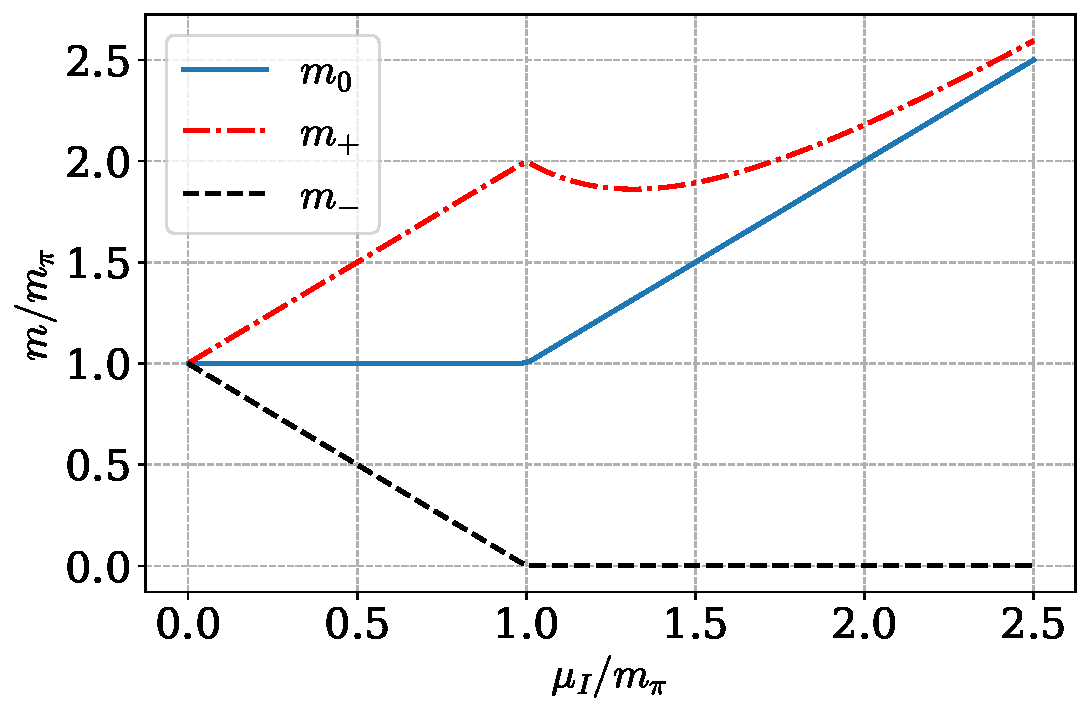
\includegraphics[width=0.7\textwidth]{../scripts/figurer/leading_order_masses.pdf}
    \caption{The masses of the three particles as functions of isosopin chemical potential. Rresults are given in units of the pion mass, $m_\pi$.}
    \label{fig: masses}
\end{figure}

With the energies of the pions, we can write the determinant of the inverse propagator as
%
\begin{equation}
    \det(D^{-1}) = (p_0^2 - E_0^2) (p_0^2 - E_+^2) (p_0^2 - E_-^2).
\end{equation}
%
The propagator and the inverse propagator in momentum space obey\footnote{One has to be careful regarding the factor $i$ in the physicist's definition of propagators. It has the consequence that $D^{-1}$ is not strictly the operator inverse of the propagator $D$.}
%
\begin{equation}
    \sum_c D_{ac}(p)D_{cb}^{-1}(p) = i \delta_{ab}
\end{equation}
%
Using this, we can solve for the propagator
%
\begin{align}
    D & = (- iD^{-1})^{-1} 
    \label{free pion propagator}
    = i
    \begin{pmatrix}
        \frac{
            p^2 - m_2^2
        }
        {
            (p_0^2 - E_+^2)(p_0^2 - E_-^2)
        } 
        & \frac{
            - ip_0m_{12}
        }
        {
            (p_0^2 - E_+^2)(p_0^2 - E_-^2)
        } & 0 \\
        \frac{
            ip_0m_{12}
        }
        {
            (p_0^2 - E_+^2)(p_0^2 - E_-^2)
        }
        & \frac{
            p^2 - m_1^2
        }
        {
            (p_0^2 - E_+^2)(p_0^2 - E_-^2)
        } & 0 \\
        0 & 0 & 
        \frac{1}{p_0^2 - E_0^2}
    \end{pmatrix}.
\end{align}




\section{Electromagnetic effects}

When including contribution from a dynamical photon field, the leading order Lagrangian is~\autocite{eckerRoleResonancesChiral1989,urechVirtualPhotonsChiral1995}
%
\begin{equation}
    \label{leading order lagrangian EM}
    \Ell_2^{\text{EM}}
    = 
    \frac{1}{4}f^2 
    \Tr{
        \nabla_\mu \Sigma \nabla^\mu \Sigma^\dagger
    }
    +
    \frac{1}{4}f^2 
    \Tr{
        \chi \Sigma^\dagger + \Sigma\chi^\dagger
    }
    +
    e^2 C
    \Tr{Q \Sigma Q \Sigma^\dagger}
\end{equation}
%
$Q$ is the quark charge matrix, which for $N_f = 2$ is
%
\begin{equation}
    \label{two-flavor charge matrix}
    Q
    =
    \frac{1}{3} 
    \begin{pmatrix}
        2 & 0 \\
        0 & -1
    \end{pmatrix}
    = 
    \frac{1}{2} \one + \frac{1}{6} \tau_3.
\end{equation}
%
$C$ and dimensionfull constant, and $\chi = 2B_0 m$, where $m$ is the quark mass matrix \autoref{two-flavor mass matrix}.
To find the electromagnetic effect on the pion mass, we assume $\mu_I = 0$.
We use the parametrization $\Sigma = \exp{i \pi_a \tau_a / f}$, and the covariant derivative is in this case
%
\begin{equation}
    \nabla_\mu \Sigma = \partial_\mu \Sigma - i e \mathcal A_\mu [Q, \Sigma].
\end{equation}
%
We expand to second order in $\pi_a/f$, which gives
%
\begin{align}
    \frac{1}{4}f^2 \Tr{\nabla_\mu \Sigma \nabla^\mu \Sigma}
    &=
    \frac{1}{2}\partial_\mu \pi_a\partial^\mu \pi_a
    + e \mathcal A^\mu (\pi_1 \partial_\mu \pi_2 -\pi_2 \partial_\mu \pi_1)
    + e^2 \mathcal A^2 (\pi_1^2 + \pi_2^2), \\
    \frac{1}{4}f^2 \Tr{\chi \Sigma^\dagger + \Sigma \chi^\dagger}
    & = \bar m^2\left(f^2 - \frac{1}{2} \pi_a \pi_a\right), \\
    \Tr{Q \Sigma Q \Sigma^\dagger}
    & = \frac{5}{9} - \frac{\pi_1^2 + \pi_2^2}{f^2}.
\end{align}
%
Inserting this into \autoref{leading order lagrangian EM}, we get
%
\begin{equation}
    \Ell_2^\text{EM}
    = \bar m^2 f^2 + \frac{5}{9}e^2 C
    + \frac{1}{2}\partial_\mu \pi_a \partial^\mu \pi_a
    - \frac{1}{2} \bar m_\pm^2 (\pi_1^2 + \pi_2^2) 
    - \frac{1}{2}\bar m^2 \pi_3^2
    + e \mathcal A^\mu (\pi_1 \partial_\mu \pi_2 -\pi_2 \partial_\mu \pi_1)
    + e^2 \mathcal A^2 (\pi_1^2 + \pi_2^2).
\end{equation}
%
where
\begin{equation}
    \bar m_\pm^2 = \bar m^2 + 2\frac{e^2}{f^2}C.
\end{equation}
%
This is the leading order electromagnetic contribution to the mass.
It only affects the $\pi_1, \pi_2$ pions, as they are linear combinations of the charged pions $\pi^\pm$, while $\pi_3 = \pi^0$, the neutral pion.
To leading order, $\bar m = m_\pi$, the neutral pion mass, and $\bar m_{\pm} = m_{\pi^{\pm}}$
From the values listed in \autoref{section: units}, we find
%
\begin{equation}
    \label{EM mass contribtuion leading order}
    \Delta m_{\pm} := \frac{e}{f}\sqrt{2C} = \sqrt{m_{\pi_\pm}^2 - m_{\pi}^2} = 35.50 \, \text{MeV}.
\end{equation}
%
This corresponds to $C = 0.3771 \, u_0 = 5.824 \cdot 10^{-5} \, \text{GeV}^4$.
We now no longer assume $\mu_I = 0$.
The zeroth-order expansion in $\pi/f$ is
%
\begin{equation}
    \Sigma = e^{i \alpha \tau_1} = \sin \alpha + i \tau_1 \cos \alpha.
\end{equation}
%
This gives the contributions
%
\begin{align}
    \Tr{\nabla_\mu \Sigma \nabla^\mu \Sigma^\dagger}
    & = 2 \sin^2\alpha\left(\mu_I^2 + 2 e \mu \mathcal A_0 + e^2\mathcal A^2 \right), \\
    \Tr{\chi \Sigma^\dagger + \Sigma \chi^\dagger}
    & =4 \bar m^2 \cos \alpha,\\
    \Tr{Q \Sigma Q \Sigma^\dagger}
    & =  \cos^2 \alpha - \frac{4}{9}.
\end{align}
%
We are interested in the static Lagrangian, the Lagrangian for $\pi_a = \mathcal A_\mu = 0$.
Inserting these terms into \autoref{leading order lagrangian EM}, we get
%
\begin{equation}
    \label{static lagrangian with EM}
    \Ell^{\text{EM}, 0}_2
    = f^2 \left[
        \frac{1}{2}\mu_I^2 \sin^2 \alpha + \bar m^2 \cos \alpha 
        + \frac{1}{2} \Delta m^2_{\pi_\pm} \left(\cos^2 \alpha - \frac{4}{9}\right)
    \right].
\end{equation}
%

